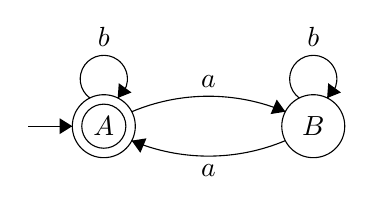
\begin{tikzpicture}[scale=0.2]
    \tikzstyle{every node}+=[inner sep=0pt]
    \draw [black] (18.3,-6.9) circle (2);
    \draw (18.3,-6.9) node {$B$};
    \draw [black] (5,-6.9) circle (2);
    \draw (5,-6.9) node {$A$};
    \draw [black] (5,-6.9) circle (1.4);
    \draw [black] (4.118,-5.114) arc (234:-54:1.5);
    \draw (5,-1.9) node [above] {$b$};
    \fill [black] (5.88,-5.11) -- (6.76,-4.76) -- (5.95,-4.17);
    \draw [black] (17.418,-5.114) arc (234:-54:1.5);
    \draw (18.3,-1.9) node [above] {$b$};
    \fill [black] (19.18,-5.11) -- (20.06,-4.76) -- (19.25,-4.17);
    \draw [black] (6.774,-5.981) arc (112.81668:67.18332:12.574);
    \fill [black] (16.53,-5.98) -- (15.98,-5.21) -- (15.59,-6.13);
    \draw (11.65,-4.5) node [above] {$a$};
    \draw [black] (16.525,-7.818) arc (-67.2022:-112.7978:12.582);
    \fill [black] (6.77,-7.82) -- (7.32,-8.59) -- (7.71,-7.67);
    \draw (11.65,-9.3) node [below] {$a$};
    \draw [black] (0.2,-6.9) -- (3,-6.9);
    \fill [black] (3,-6.9) -- (2.2,-6.4) -- (2.2,-7.4);
    \end{tikzpicture}